\documentclass{standalone}
\usepackage{tikz}
\usetikzlibrary{patterns, positioning}
\usepackage[sfdefault]{ClearSans} %% option 'sfdefault' activates Clear Sans as the default text font
\usepackage[T1]{fontenc}

\begin{document}
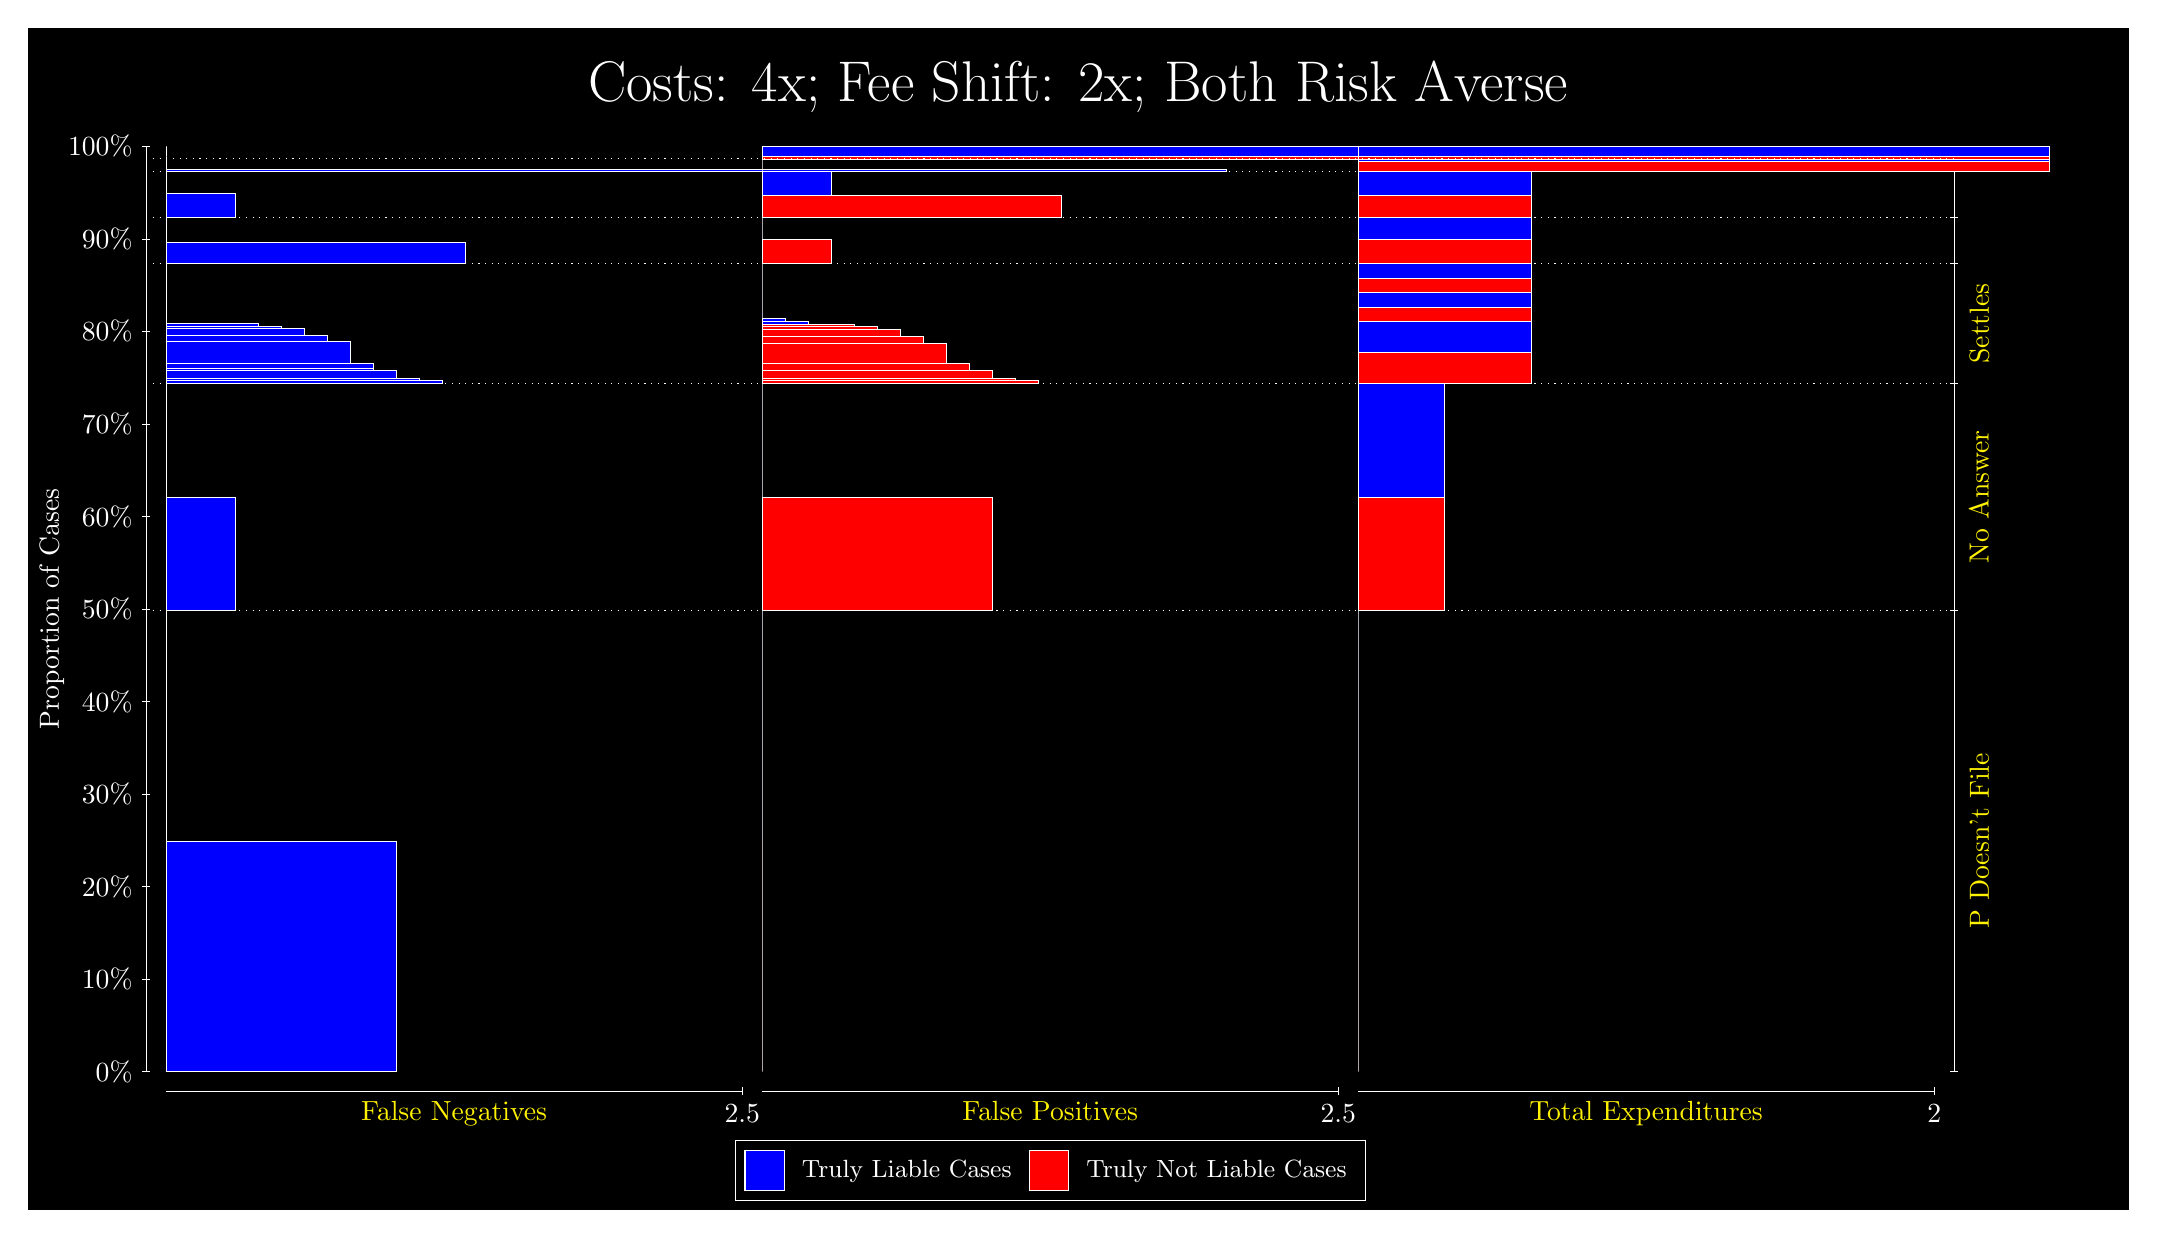
\begin{tikzpicture}
\draw[fill=black] (0,0) rectangle (26.667,15);
\draw[text=white] (0,13.5) rectangle (26.667,15) node[midway] {\huge Costs: 4x; Fee Shift: 2x; Both Risk Averse};
\draw[white, very thin] (1.5,1.75) -- (1.5,13.5);
\node[rotate=90, text=white, anchor=center] at (0.3, 7.625) {Proportion of Cases};
\draw[white, very thin] (1.45,1.75) -- (1.55,1.75);
\node[text=white, anchor=east] at (1.45, 1.75) {0\%};
\draw[white, very thin] (1.45,2.925) -- (1.55,2.925);
\node[text=white, anchor=east] at (1.45, 2.925) {10\%};
\draw[white, very thin] (1.45,4.1) -- (1.55,4.1);
\node[text=white, anchor=east] at (1.45, 4.1) {20\%};
\draw[white, very thin] (1.45,5.275) -- (1.55,5.275);
\node[text=white, anchor=east] at (1.45, 5.275) {30\%};
\draw[white, very thin] (1.45,6.45) -- (1.55,6.45);
\node[text=white, anchor=east] at (1.45, 6.45) {40\%};
\draw[white, very thin] (1.45,7.625) -- (1.55,7.625);
\node[text=white, anchor=east] at (1.45, 7.625) {50\%};
\draw[white, very thin] (1.45,8.8) -- (1.55,8.8);
\node[text=white, anchor=east] at (1.45, 8.8) {60\%};
\draw[white, very thin] (1.45,9.975) -- (1.55,9.975);
\node[text=white, anchor=east] at (1.45, 9.975) {70\%};
\draw[white, very thin] (1.45,11.15) -- (1.55,11.15);
\node[text=white, anchor=east] at (1.45, 11.15) {80\%};
\draw[white, very thin] (1.45,12.325) -- (1.55,12.325);
\node[text=white, anchor=east] at (1.45, 12.325) {90\%};
\draw[white, very thin] (1.45,13.5) -- (1.55,13.5);
\node[text=white, anchor=east] at (1.45, 13.5) {100\%};

\draw[white, very thin] (24.457,1.75) -- (24.457,13.5);
\draw[white, very thin] (24.407,1.75) -- (24.507,1.75);
\node[anchor=west] at (24.407, 1.75) {};
\draw[white, very thin] (24.407,7.6052) -- (24.507,7.6052);
\node[anchor=west] at (24.407, 7.6052) {};
\draw[white, very thin] (24.407,10.49) -- (24.507,10.49);
\node[anchor=west] at (24.407, 10.49) {};
\draw[white, very thin] (24.407,12.01) -- (24.507,12.01);
\node[anchor=west] at (24.407, 12.01) {};
\draw[white, very thin] (24.407,12.595) -- (24.507,12.595);
\node[anchor=west] at (24.407, 12.595) {};
\draw[white, very thin] (24.407,13.181) -- (24.507,13.181);
\node[anchor=west] at (24.407, 13.181) {};
\draw[white, very thin] (24.407,13.34) -- (24.507,13.34);
\node[anchor=west] at (24.407, 13.34) {};
\draw[white, very thin] (24.407,13.5) -- (24.507,13.5);
\node[anchor=west] at (24.407, 13.5) {};

\draw[white, very thin, fill=blue] (1.75,1.75) rectangle (4.6775,4.6776);
\draw[white, very thin, fill=red] (1.75,4.6776) rectangle (1.75,7.6052);
\draw[white, very thin, fill=blue] (1.75,7.6052) rectangle (2.6283,9.0474);
\draw[white, very thin, fill=red] (1.75,9.0474) rectangle (1.75,10.49);
\draw[white, very thin, fill=blue] (1.75,10.49) rectangle (5.2631,10.524);
\draw[white, very thin, fill=blue] (1.75,10.524) rectangle (4.9703,10.555);
\draw[white, very thin, fill=blue] (1.75,10.555) rectangle (4.6775,10.658);
\draw[white, very thin, fill=blue] (1.75,10.658) rectangle (4.3848,10.676);
\draw[white, very thin, fill=blue] (1.75,10.676) rectangle (4.3848,10.748);
\draw[white, very thin, fill=blue] (1.75,10.748) rectangle (4.092,11.019);
\draw[white, very thin, fill=blue] (1.75,11.019) rectangle (3.7993,11.099);
\draw[white, very thin, fill=blue] (1.75,11.099) rectangle (3.5065,11.19);
\draw[white, very thin, fill=blue] (1.75,11.19) rectangle (3.2138,11.22);
\draw[white, very thin, fill=blue] (1.75,11.22) rectangle (2.921,11.254);
\draw[white, very thin, fill=red] (1.75,11.254) rectangle (1.75,12.01);
\draw[white, very thin, fill=blue] (1.75,12.01) rectangle (5.5558,12.287);
\draw[white, very thin, fill=red] (1.75,12.287) rectangle (1.75,12.595);
\draw[white, very thin, fill=blue] (1.75,12.595) rectangle (2.6283,12.9);
\draw[white, very thin, fill=red] (1.75,12.9) rectangle (1.75,13.181);
\draw[white, very thin, fill=blue] (1.75,13.181) rectangle (15.217,13.213);
\draw[white, very thin, fill=red] (1.75,13.213) rectangle (1.75,13.34);
\draw[white, very thin, fill=red] (1.75,13.34) rectangle (1.75,13.372);
\draw[white, very thin, fill=blue] (1.75,13.372) rectangle (1.75,13.5);
\draw[white, very thin, fill=red] (9.3189,1.75) rectangle (9.3189,4.6777);
\draw[white, very thin, fill=blue] (9.3189,4.6777) rectangle (9.3189,7.6052);
\draw[white, very thin, fill=red] (9.3189,7.6052) rectangle (12.246,9.0475);
\draw[white, very thin, fill=blue] (9.3189,9.0475) rectangle (9.3189,10.49);
\draw[white, very thin, fill=red] (9.3189,10.49) rectangle (12.832,10.523);
\draw[white, very thin, fill=red] (9.3189,10.523) rectangle (12.539,10.554);
\draw[white, very thin, fill=red] (9.3189,10.554) rectangle (12.246,10.654);
\draw[white, very thin, fill=red] (9.3189,10.654) rectangle (11.954,10.741);
\draw[white, very thin, fill=red] (9.3189,10.741) rectangle (11.661,11.005);
\draw[white, very thin, fill=red] (9.3189,11.005) rectangle (11.368,11.086);
\draw[white, very thin, fill=red] (9.3189,11.086) rectangle (11.075,11.18);
\draw[white, very thin, fill=red] (9.3189,11.18) rectangle (10.783,11.211);
\draw[white, very thin, fill=red] (9.3189,11.211) rectangle (10.49,11.246);
\draw[white, very thin, fill=blue] (9.3189,11.246) rectangle (9.9044,11.279);
\draw[white, very thin, fill=blue] (9.3189,11.279) rectangle (9.6116,11.31);
\draw[white, very thin, fill=blue] (9.3189,11.31) rectangle (9.3189,12.01);
\draw[white, very thin, fill=red] (9.3189,12.01) rectangle (10.197,12.319);
\draw[white, very thin, fill=blue] (9.3189,12.319) rectangle (9.3189,12.595);
\draw[white, very thin, fill=red] (9.3189,12.595) rectangle (13.125,12.876);
\draw[white, very thin, fill=blue] (9.3189,12.876) rectangle (10.197,13.181);
\draw[white, very thin, fill=red] (9.3189,13.181) rectangle (9.3189,13.307);
\draw[white, very thin, fill=blue] (9.3189,13.307) rectangle (9.3189,13.34);
\draw[white, very thin, fill=red] (9.3189,13.34) rectangle (22.786,13.372);
\draw[white, very thin, fill=blue] (9.3189,13.372) rectangle (19.858,13.5);
\draw[white, very thin, fill=red] (16.888,1.75) rectangle (16.888,4.6777);
\draw[white, very thin, fill=blue] (16.888,4.6777) rectangle (16.888,7.6052);
\draw[white, very thin, fill=red] (16.888,7.6052) rectangle (17.986,9.0475);
\draw[white, very thin, fill=blue] (16.888,9.0475) rectangle (17.986,10.49);
\draw[white, very thin, fill=red] (16.888,10.49) rectangle (19.083,10.885);
\draw[white, very thin, fill=blue] (16.888,10.885) rectangle (19.083,11.278);
\draw[white, very thin, fill=red] (16.888,11.278) rectangle (19.083,11.456);
\draw[white, very thin, fill=blue] (16.888,11.456) rectangle (19.083,11.643);
\draw[white, very thin, fill=red] (16.888,11.643) rectangle (19.083,11.825);
\draw[white, very thin, fill=blue] (16.888,11.825) rectangle (19.083,12.01);
\draw[white, very thin, fill=red] (16.888,12.01) rectangle (19.083,12.319);
\draw[white, very thin, fill=blue] (16.888,12.319) rectangle (19.083,12.595);
\draw[white, very thin, fill=red] (16.888,12.595) rectangle (19.083,12.876);
\draw[white, very thin, fill=blue] (16.888,12.876) rectangle (19.083,13.181);
\draw[white, very thin, fill=red] (16.888,13.181) rectangle (25.67,13.307);
\draw[white, very thin, fill=blue] (16.888,13.307) rectangle (25.67,13.34);
\draw[white, very thin, fill=red] (16.888,13.34) rectangle (25.67,13.372);
\draw[white, very thin, fill=blue] (16.888,13.372) rectangle (25.67,13.5);
\draw[white, dotted] (1.5,7.6052) -- (24.457,7.6052);
\draw[white, dotted] (1.5,10.49) -- (24.457,10.49);
\draw[white, dotted] (1.5,12.01) -- (24.457,12.01);
\draw[white, dotted] (1.5,12.595) -- (24.457,12.595);
\draw[white, dotted] (1.5,13.181) -- (24.457,13.181);
\draw[white, dotted] (1.5,13.34) -- (24.457,13.34);
\draw[white, very thin] (1.75,1.5) -- (9.0689,1.5);
\node[text=yellow, anchor=north] at (5.4094, 1.5) {False Negatives};
\draw[white, very thin] (9.0689,1.45) -- (9.0689,1.55);
\node[text=white, anchor=north] at (9.0689, 1.45) {2.5};

\draw[white, very thin] (9.3189,1.5) -- (16.638,1.5);
\node[text=yellow, anchor=north] at (12.978, 1.5) {False Positives};
\draw[white, very thin] (16.638,1.45) -- (16.638,1.55);
\node[text=white, anchor=north] at (16.638, 1.45) {2.5};

\draw[white, very thin] (16.888,1.5) -- (24.207,1.5);
\node[text=yellow, anchor=north] at (20.547, 1.5) {Total Expenditures};
\draw[white, very thin] (24.207,1.45) -- (24.207,1.55);
\node[text=white, anchor=north] at (24.207, 1.45) {2};

\node[text=yellow, centered, rotate=90] at (24.777, 4.6776) {P Doesn't File};
\node[text=yellow, centered, rotate=90] at (24.777, 9.0475) {No Answer};
\node[text=yellow, centered, rotate=90] at (24.777, 11.25) {Settles};





\draw (12.978300999999998,1.5) node[draw=none] (baseCoordinate) {};
\begin{scope}[align=center]
        \matrix[scale=0.5, draw=white, below=0.5cm of baseCoordinate, nodes={draw}, column sep=0.1cm]{
            \node[rectangle, draw, minimum width=0.5cm, minimum height=0.5cm, fill=blue] {}; &
            \node[draw=none, font=\small, text=white] (B) {Truly Liable Cases}; &
            \node[rectangle, draw, minimum width=0.5cm, minimum height=0.5cm, fill=red] {}; &
            \node[draw=none, font=\small, text=white] (B) {Truly Not Liable Cases}; \\
            };
\end{scope}

\end{tikzpicture}
\end{document}